%template1.tex
%The following LaTeX source file represents the simplest kind of slide presentation; no overlays, no included graphics. Substitute your favorite style for ``pascal''. To create the PDF file template1.pdf, (1) be sure to use the prosper class, then (2) execute the command latex template1.tex, and (3) the command dvipdf template1.dvi.

%%%%%%%%%%%%%%%%%%%%%%%%%%%%%%% template1.tex %%%%%%%%%%%%%%%%%%%%%%%%%%%%%%%%%%%
\documentclass[a4paper,blends,pdf,colorBG,slideColor]{prosper}
% definitions for slides for CSC544
% Lutz Hamel, (c) 2007

\hypersetup{pdfpagemode=FullScreen}

\usepackage{amssymb}
\usepackage{latexsym}
\usepackage{amsmath}
%\usepackage[usenames]{color}
\usepackage{xypic}


\newcommand{\term}[1]{\ensuremath{\mbox{\bf #1}}}
\newcommand{\nonterm}[1]{\ensuremath{\mbox{#1}}}
\newcommand{\ifstmt}[3]{\ensuremath{{\bf if}\; {#1}\;{\bf then}\;{#2}\;{\bf else}\;{#3}\;\term{end}}}
\newcommand{\whilestmt}[2]{\ensuremath{{\bf while}\; {#1}\;{\bf do}\;{#2}\; \term{end}}}
\newcommand{\funcstmt}[3]{\ensuremath{{\bf fun}\; {#1}\; {\bf is}\; {#2} \; {\bf return}\; {#3}}}
\newcommand{\syntaxset}[1]{\ensuremath{\mbox{\bf #1}}}
\newcommand{\orbar}{\;|\;}
\newcommand{\bs}[1]{\begin{slide}{#1}\ptsize{8}}
\newcommand{\es}{\end{slide}}
\newcommand{\co}{\,\colon\;}
\newcommand{\pair}[2]{\ensuremath{\langle {#1}, {#2} \rangle}}
\newcommand{\encode}[1]{\ensuremath{\langle {#1} \rangle}}
\newcommand{\mytab}{\makebox[.15in]{}}
%\newcommand{\abs}[1]{{\mid{#1}\mid}}
\newcommand{\abs}[1]{{|{#1}|}}
\newcommand{\ol}[1]{\overline{#1}}

\newcommand{\qaccept}{\ensuremath{q_{\mbox{\tiny accept}}}}
\newcommand{\qreject}{\ensuremath{q_{\mbox{\tiny reject}}}}
\newcommand{\accept}{{\em accept}}
\newcommand{\reject}{{\em reject}}

\newcommand{\machine}[1]{
	\begin{quote}
	{#1}
	\end{quote}
	}

\newcommand{\fdef}[1]{
	\begin{center}
	\fbox{
	\begin{minipage}{3.5in}
	{\bf Definition:}
	{#1}
	\end{minipage}
	}
	\end{center}
	}

\newcommand{\ftheorem}[1]{
	\begin{center}
	\fbox{
	\begin{minipage}{3.5in}
	{\bf Theorem:}
	{#1}
	\end{minipage}
	}
	\end{center}
	}

\newcommand{\flemma}[1]{
	\begin{center}
	\fbox{
	\begin{minipage}{3.5in}
	{\bf Lemma:}
	{#1}
	\end{minipage}
	}
	\end{center}
	}


\newcommand{\fframe}[1]{
	\begin{center}
	\fbox{
	\begin{minipage}{3.5in}
	{#1}
	\end{minipage}
	}
	\end{center}
	}

\newcommand{\nframe}[1]{
	\begin{center}
	\begin{minipage}{3.5in}
	{#1}
	\end{minipage}
	\end{center}
	}

\begin{document}


\bs{Turing Machines}
A Turing machine is a FA with an infinite tape as memory.

\begin{center}

\includegraphics[height=20mm]{images/tm_0001.eps}
\end{center}

Initially, the tape contains the input to the Turing machine.

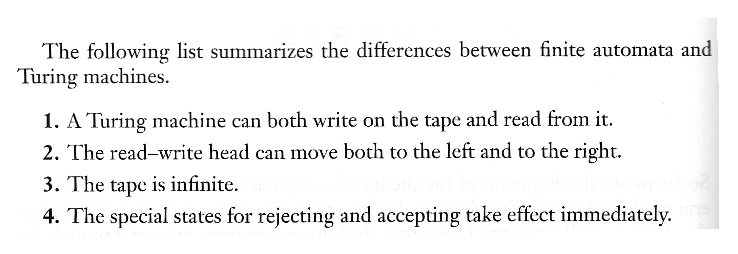
\includegraphics[height=30mm]{images/tm_0002.eps}
\es

\bs{Church-Turing Thesis}

Why do we study Turing machines?

\begin{center}
\vspace{.5in}
\fbox{
\begin{minipage}{3in}
\begin{center}
Intuitive Notion of Algorithms


{\em equals}

Turing Machine Algorithms
\end{center}
\end{minipage}
}
\end{center}
\vspace{.5in}
This equivalence cannot be proved but up to now no algorithm has been found
that could not be implemented on a Turing machine.
\es


\bs{Turing Machines}
{\bf Example:} Construct a TM, call it $M_1$, that tests whether a string
is a member of the language $B = \{u\#u \mid u \in \{0,1\}^*\}$.  That is,
if some string $w \in B$ then {\em accept} otherwise {\em reject}.
Assume that the string $w$ is loaded on the tape before the machine runs;
the tape will look something like this for $w = 101\#101$,
\[
1\;0\;1\;\#\;1\;0\;1\;\sqcup\ldots
\]
Algorithm:

$M_1 = $ ``On input string $w$:
\begin{enumerate}
\item Zig-zag across the tape to corresponding positions on either side of the \# symbol
to check whether these positions contain the same symbol.  If they do not, or if no \#
is found, {\em reject}.  Cross off symbols as they are checked to keep track of which symbols correspond.

\item When all symbols to the left of the \# have been crossed off, check for any remaining symbols to the right of the \#. If any symbols remain, {\em reject}; otherwise, {\em accept}."
\end{enumerate}
\es

\bs{Turing Machines}
\begin{center}
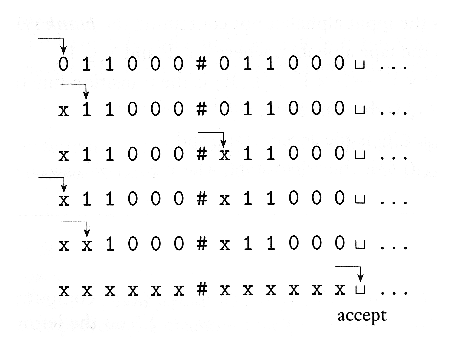
\includegraphics[height=60mm]{images/tm-computing.eps}
\end{center}
\es

\bs{Turing Machines}
{\bf Example:} Construct a machine $M$ that tests whether a string belongs to the language
\[
L = \{ a^ib^jc^k \mid i,j,k \ge 0 \wedge i=k=j\}.
\]
Algorithm:

$M = $ ``On input string $w$:
\begin{enumerate}
\item Scan across the tape and make sure the $a$'s, $b$'s, and $c$'s are properly ordered.
\item Scan across the tape and count the numbers of $a$'s, $b$'s, and $c$'s.
 If the numbers do not match, {\em reject}.  
\item Otherwise, {\em accept}."
\end{enumerate}

\es

\bs{Formal Definition}
\begin{center}
\fbox{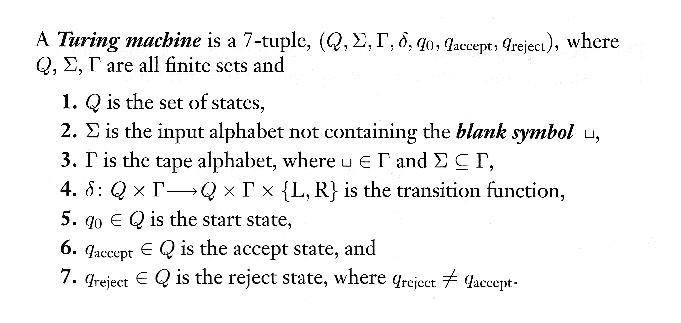
\includegraphics[height=40mm]{images/tm-def.eps}}
\end{center}

{\bf NOTE:} A TM computes until it enters either an accept or reject state.


\es

\bs{$M_1$ Revisited}
$L(M_1) = \{u\#u \mid u \in \{0,1\}^*\}$

\begin{center}
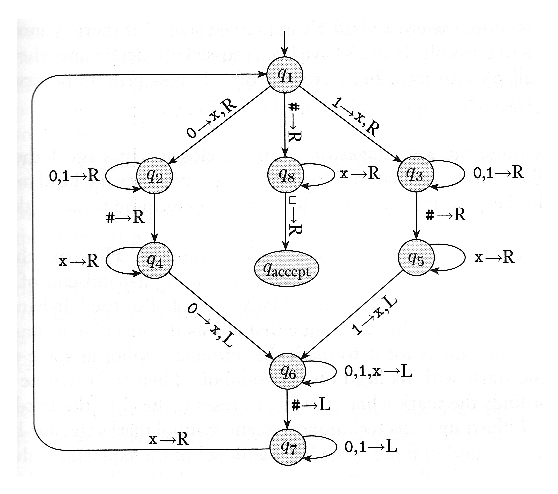
\includegraphics[height=40mm]{images/tm-m1.eps}
\end{center}

{\bf NOTE:} Transition into $q_{reject}$ are implicit on symbols not appearing
at states.
\es


\bs{Configurations}

{\bf NOTE:} The current state, the current tape contents, and the current head location
is called a {\bf\em configuration}.

\begin{description}
\item[start configuration:] the TM is in state $q_0$ with the tape head pointing
to the leftmost position.
\item[halting configuration:] a state in which the machine is either in an
accept state ({\bf accepting configuration}) or in a reject state ({\bf rejecting configuration})
\end{description}
\es

\bs{TM's \& Languages}
Three outcomes are possible when a TM computes: accept, reject, or loop.

This lead to the following definitions.

\begin{center}
\fbox{
\begin{minipage}{3in}
{\bf Definition:} Call a language {\bf\em Turing-recognizable} if some
Turing machine recognizes it.
\end{minipage}
}
\end{center}

The problem with TM's that recognize a language is that they might loop
on some inputs.  We prefer machines that always halt.  We call such machines
{\bf\em deciders}.

\fdef{Call a language {\bf\em Turing-decidable} or simply {\bf\em decidable} if some Turing machine decides it.}

Deciders will answer definitively on the question whether a string belongs to a
language or not.

{\bf NOTE:} Every decidable language is Turing-recognizable (why?).

\es

\bs{Language Hierarchy}
\vspace{.5in}
\begin{center}
\includegraphics[height=50mm]{images/tm-hierarchy.eps}
\end{center}
\es


\bs{Generators}

The generators associated with TMs are {\em unconstrained grammars} or {\em type-0} grammars.

Recall that a type-0 grammar $G=(V,\Sigma,R,s)$ is a grammar where the shape of each rule in $R$ is 
completely unrestricted:
\[
\alpha \rightarrow \beta
\]
with $\alpha, \beta \in (V\cup \Sigma)^*$.
\es

\bs{Generators}
{\bf Example:}  The non-context-free language
\[
L= \{a^ib^jc^k \mid i,j,k \ge 0\}
\]
is generated by the following type-0 grammar $G = (V,\Sigma,R,s)$,
\begin{itemize}
\item $V = \{S,B\}$,
\item $\Sigma = \{a,b,c\}$,
\item The rule set $R$ is as follows,
\begin{eqnarray*}
S &\rightarrow& a B S c\\
S &\rightarrow& a b c\\
S &\rightarrow& \epsilon\\
Ba &\rightarrow& a B\\
Bb &\rightarrow& b b
\end{eqnarray*}
\item $s = S$.
\end{itemize}
\es

\bs{Generators}
{\bf Observation:} Unrestricted term rewriting systems are {\em Turing complete}, that is they can express
the same computations that Turing machines can express.\footnote{Perhaps not a surprise, because Algebra,
Calculus etc. are all just very fancy rewriting systems.}
\footnote{Later on we will discuss an interesting term rewriting system called the lambda calculus which
basically models computing with functions.}
\es

\bs{Assignment}
Assignment \#2 -- see web
\es

\end{document}
%%%%%%%%%%%%%%%%%%%%%%%%%%% end of template1.tex %%%%%%%%%%%%%%%%%%%%%%%%%%%%%%%%

